\section{\scshape Work plan}\label{sec:workplan}

\subsection{Tasks}
\begin{frame}{Tasks}
	\begin{footnotesize}
		\begin{itemize}
			\item Use cases definition (1 month)
			\item Review of state of the art (1 month)
			\item Evaluation and selection of hardware for testing platforms (2 month)
			\item Creation of perception and learning datasets (2 month)
			\item Definition of software architecture (3 months)
			\item Knowledge / skill representation (3 months)
			\item Extraction of assembly knowledge from SOPs (3 months)
			\item Assembly operations from structured knowledge / assembly skills (3 months)
			\item Learning of new assembly operations from human demonstration (5 months)
			\item Immersive human-robot cooperation using projection mapping (2 months)
			\item Validation of assembly system in industrial conditions (4 months)
			\item Writing of thesis (7 months)
		\end{itemize}
	\end{footnotesize}
\end{frame}

\subsection{Gantt chart}
\begin{frame}{Gantt chart}
	\begin{figure}
		\centering
		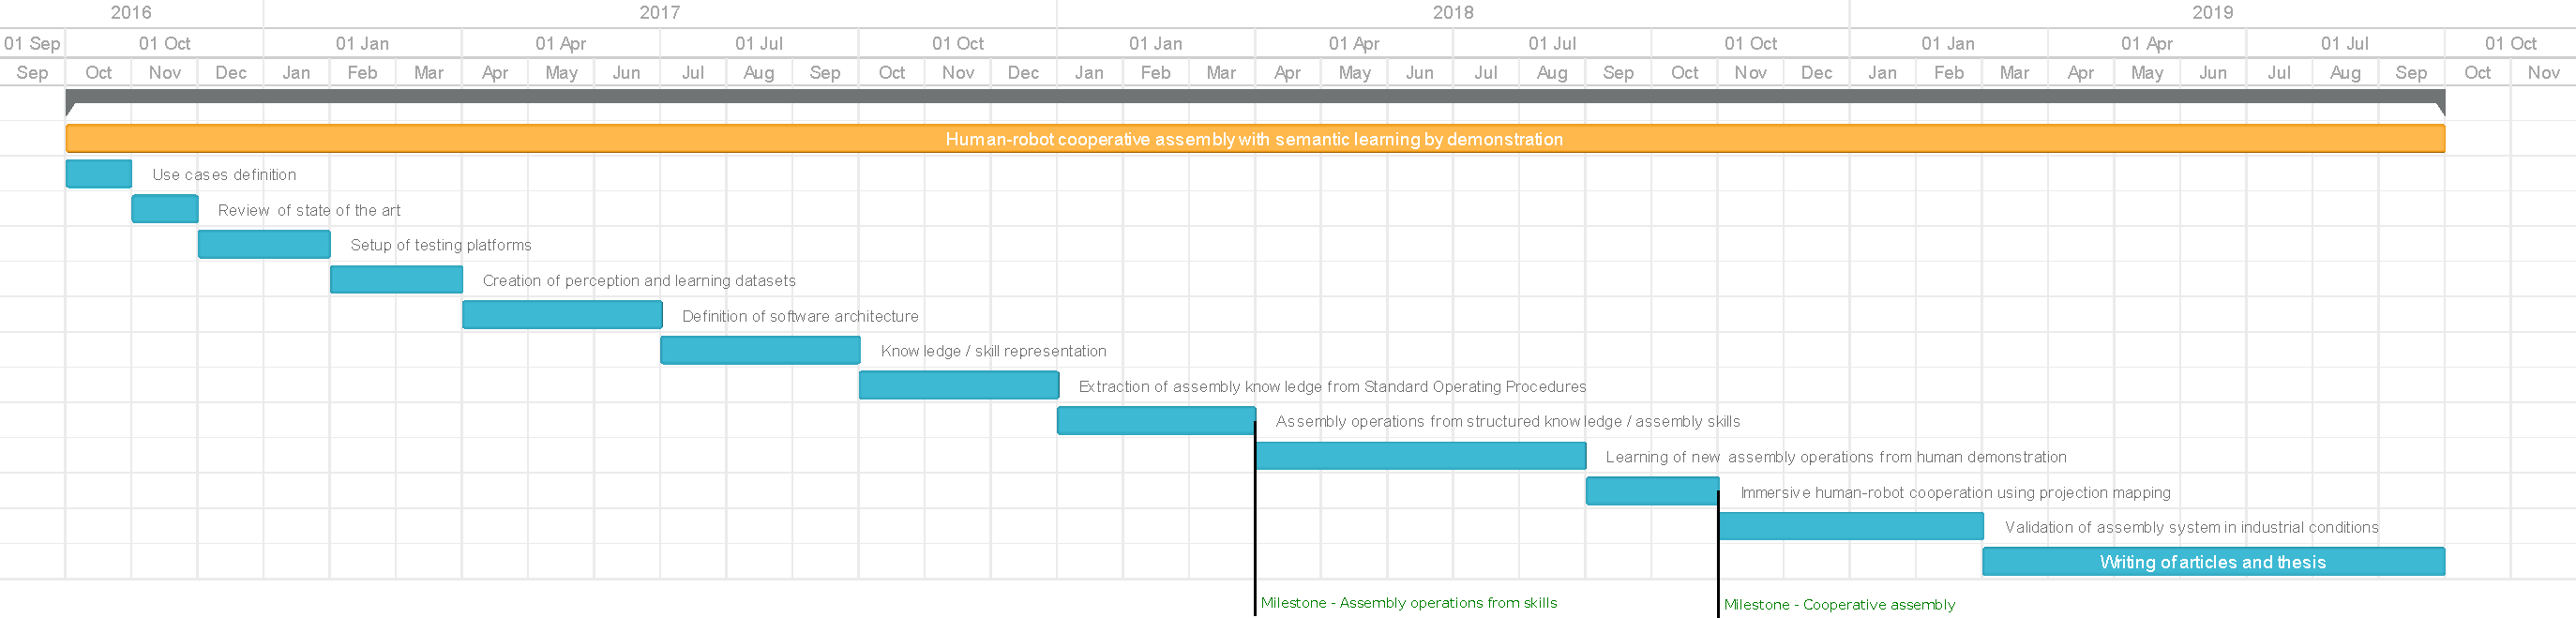
\includegraphics[width=\linewidth]{gantt-chart}
		\caption{Gantt chart}
	\end{figure}
\end{frame}
